% -- Iniciando o documento --
\documentclass[
	12pt,		% Tamanho da fonte
	a4paper,	% Tamanho do papel
	english,	% Idioma adicional
	brazil,		% Idioma principal
	openright,	% Capitulos começam em pag impar
	oneside		% Apenas 1 página por folha
	]{abntex2}

\usepackage{lmodern}			% Usa a fonte Latin Modern
\usepackage[T1]{fontenc}		% Selecao de codigos de fonte.
\usepackage[utf8]{inputenc}		% Codificacao do documento
\usepackage{lastpage}			% Usado pela Ficha catalográfica
\usepackage{indentfirst}		% Indenta o primeiro parágrafo de cada seção.
\usepackage{color}				% Controle das cores
\usepackage{xcolor}
\usepackage{graphicx}			% Inclusão de gráficos
\usepackage{microtype} 			% para melhorias de justificação
\usepackage{lipsum}				% para geração de dummy text
\usepackage{geometry}			% para alteração no layout das páginas
\usepackage{lscape}             % colocar páginas na horizontal compativel com longtable e supertabular.
\usepackage{bookmark}
\usepackage{caption}            % adiciona \caption*{d} para criar fontes em imagens.
\usepackage{float}				% para uso no posicionamento de imagens
\usepackage{pdfpages}
\usepackage{minibox}
\usepackage{listings}
\usepackage{multirow}           % Habilita o Merge de celulas na table

% ---
% Alterações no modelo original da abnTex2
% ---
% Impressão da Capa
\renewcommand{\imprimircapa}{%
  \begin{capa}%
    \center
    \ABNTEXchapterfont\large\imprimirinstituicao\\
    \vspace{5cm}
    \imprimirautor

    \vfill
    \begin{center}
    \ABNTEXchapterfont\bfseries\LARGE\imprimirtitulo
    \end{center}
    \vfill

    \large\imprimirlocal

    \large\imprimirdata

    \vspace*{1cm}
  \end{capa}
}
% ---
% Alteração na assinatura dos componentes da banca
\setlength{\ABNTEXsignwidth}{10cm}

\geometry{
 a4paper,
 bottom=2cm,
 top=3cm,
 left=3cm,
 right=2cm
}

% ---
% Configura layout para elementos textuais
\renewcommand{\textual}{%
  \pagestyle{plain}%abntheadings
  %\nouppercaseheads%
  \bookmarksetup{startatroot}%
  \pagenumbering{arabic}
}

\renewcommand{\pretextual}{%
  \pagestyle{plain}
  \pagenumbering{Roman}
}

%%% -----
%%% Formato de cabeçalho/rodapé romano nos elementos pré-textuais
%%% -----

%% Novo estilo
\makepagestyle{estilo_pretextual} %%% escolha um nome
  %\makeevenhead{estilo_pretextual}{}{}{\ABNTEXfontereduzida \textbf \thepage}
  \makeoddhead{estilo_pretextual}{}{}{\ABNTEXfontereduzida \textbf \thepage}

%% Customiza comando \pretextual
\renewcommand{\pretextual}{
  \pagenumbering{Roman} %%% ou \pagenumbering{Roman}
  \aliaspagestyle{chapter}{estilo_pretextual}% customizing chapter pagestyle
  \pagestyle{estilo_pretextual}
  \aliaspagestyle{cleared}{empty}
  \aliaspagestyle{part}{estilo_pretextual}
}

% ---
% Ajusta a marca \textual para que a numeração volte a ser arábica
% nos elementos textuais
\let\oldtextual\textual        % copia o comando \textual anterior para \oldtextual
\renewcommand{\textual}{%
  \pagestyle{plain}%abntheadings
  %\nouppercaseheads%
  \aliaspagestyle{chapter}{plain}
  \bookmarksetup{startatroot}%
  \pagenumbering{arabic}
}
% ---

\makeatletter
\renewcommand*{\ps@plain}{%
  \let\@mkboth\@gobbletwo
  \let\@oddhead\@empty
  \def\@oddfoot{%
    \reset@font
    \hfil
    \thepage
    % \hfil % removed for aligning to the right
  }%
  \let\@evenhead\@empty
  \let\@evenfoot\@oddfoot
}
\makeatother

% ---
% Pacotes de citações
% ---
\usepackage[brazilian, hyperpageref]{backref}	 % Paginas com as citações na bibl
\usepackage[alf]{abntex2cite}	% Citações padrão ABNT



% ---
% CONFIGURAÇÕES DE PACOTES
% ---

% ---
% Configurações do pacote backref
% Usado sem a opção hyperpageref de backref
\renewcommand{\backrefpagesname}{Citado na(s) página(s):~}
% Texto padrão antes do número das páginas
\renewcommand{\backref}{}
% Define os textos da citação
\renewcommand*{\backrefalt}[4]{
	\ifcase #1 %
		Nenhuma citação no texto.%
	\or
		Citado na página #2.%
	\else
		Citado #1 vezes nas páginas #2.%
	\fi}%
% ---

% ---
% Informações de dados para CAPA e FOLHA DE ROSTO
% ---
\titulo{Titulo do TG}

\autor{Nome Completo do Autor}
\local{São José dos Campos}
\data{\the\year}

\orientador{Titulo do orientador. Nome do Orientador}
\coorientador{Titulo do coorientador. Nome do coorientador}

\instituicao{%
  FACULDADE DE TECNOLOGIA DE SÃO JOSÉ DOS CAMPOS
  \par
  FATEC PROFESSOR JESSEN VIDAL}

\tipotrabalho{Trabalho de Graduação}

\newcommand{\disciplina}{Nome da Disciplina}

\preambulo{Trabalho de Graduação apresentado à Faculdade de Tecnologia São José dos Campos, como parte dos requisitos necessários para a obtenção do título de Tecnólogo em \disciplina.}

% Comandos para a folha de catalogacao
\newcommand{\cursoRef}{Curso de Tecnologia em \disciplina}
\newcommand{\instituicaoRef}{FATEC de S\~ao Jos\'e dos Campos: Professor Jessen Vidal}
\newcommand{\sobrenomeRef}{Sobrenome referência}
\newcommand{\nomeRef}{Nomes referência}
\newcommand{\rgRef}{00.000.000-0} % Número do RG

% informações do PDF
\makeatletter
\hypersetup{
     	%pagebackref=true,
		pdftitle={\@title},
		pdfauthor={\@author},
    	pdfsubject={\imprimirpreambulo},
	    pdfcreator={LaTeX with abnTeX2},
		pdfkeywords={abnt}{latex}{abntex}{abntex2}{trabalho acadêmico},
		colorlinks=true,       		% false: boxed links; true: colored links
    	linkcolor=blue,          	% color of internal links
    	citecolor=blue,        		% color of links to bibliography
    	filecolor=magenta,      		% color of file links
		urlcolor=blue,
		bookmarksdepth=4
}
\makeatother

% ---
% Espaçamentos entre linhas e parágrafos
% ---
\setlength{\parindent}{1.3cm} % Tamanho do parágrafo

% Controle do espaçamento entre um parágrafo e outro:
\setlength{\parskip}{0.2cm}  % tente também \onelineskip

% ---
% compila o indice
% ---
\makeindex
% ---

% ----
% Início do documento
% ----
\begin{document}
\pretextual
\selectlanguage{brazil}
\frenchspacing % Retira espaço extra obsoleto entre as frases

% ---
% Configuring all citations
\citeoption{abnt-etal-list=0}
\citeoption{abnt-last-names=abnt}
\citeoption{abnt-full-initials=yes}
% ---

% ---
% Configuring listing code
% See references on internet
% ---
\lstdefinestyle{customc}{
  belowcaptionskip=1\baselineskip,
  breaklines=true,
  %frame=L,
  xleftmargin=\parindent,
  language=C,
  numbers=left,
  showstringspaces=false,
  frame=single,
  basicstyle=\footnotesize\ttfamily,
  keywordstyle=\bfseries\color{green!40!black},
  commentstyle=\itshape\color{purple!40!black},
  identifierstyle=\color{blue},
  stringstyle=\color{orange},
}

\lstset{escapechar=@,style=customc}

% ---

% ---
% Capa
% ---
\imprimircapa
% ---

% ---
% Folha de rosto
% (o * indica que haverá a ficha bibliográfica)
% ---
\thispagestyle{empty}
\imprimirfolhaderosto
% ---

% ---
% Inserir a ficha bibliografica
% ---

\begin{fichacatalografica}
    %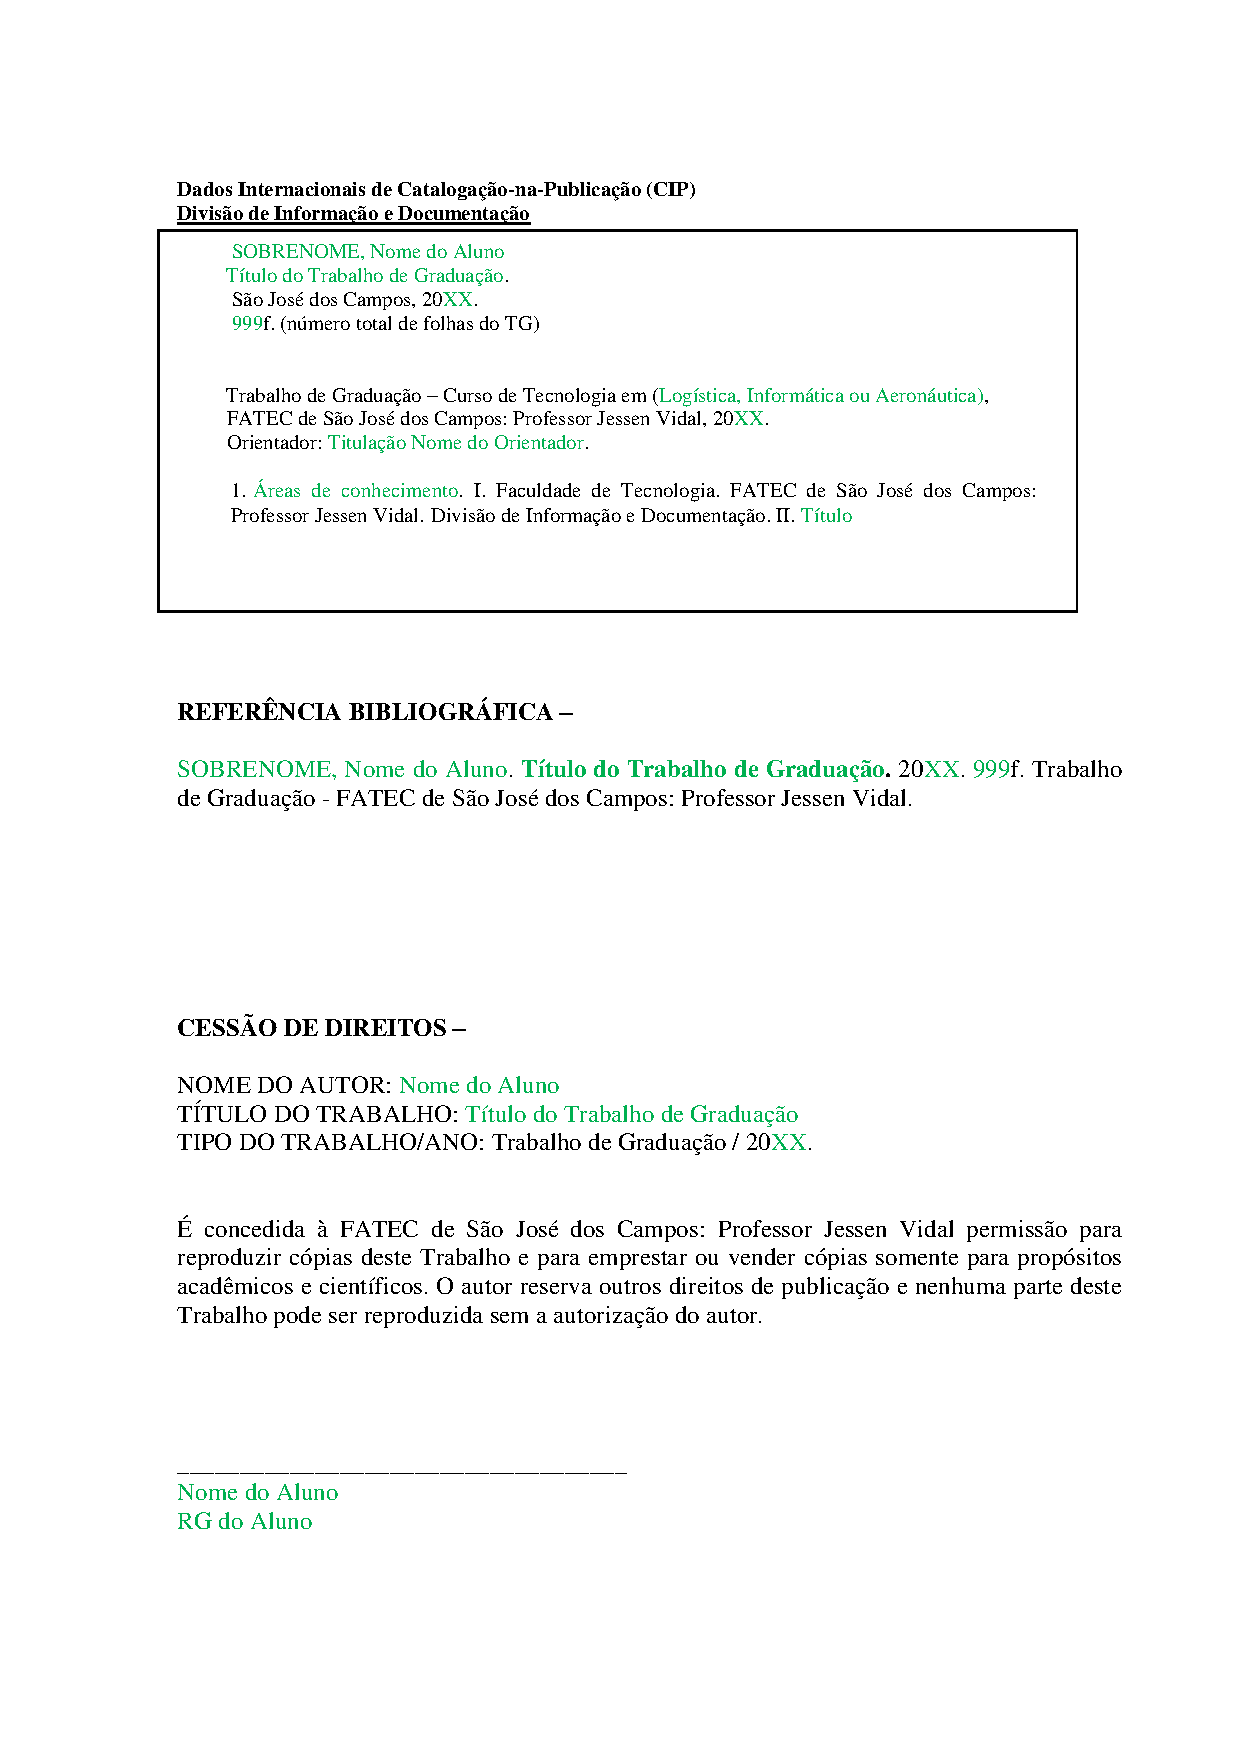
\includepdf{./testFicha}
    %%%%%%%%%%%%%
%
% Do not Edit this file!
%
%%%%%%%%%%%%%

\noindent\textbf{Dados Internacionais de Catalogação-na-Publicação (CIP)\\
Divisão de Informação e Documentação}

%\noindent\minibox[frame]{%
%    \indent INOUE, Marcos Hideki \\
%    \indent \imprimirtitulo \\
%    \indent \imprimirlocal, \the\year \\
%    \indent \pageref{LastPage}f. \\
%    \\ \\
%    \indent \imprimirtipotrabalho \-m \cursoRef \\
%    \indent \instituicaoRef, \the\year \\
%    \indent Orientador: \imprimirorientador \\
%    \indent Coorientador: \imprimircoorientador \\
%    \\
%    \indent \'Areas de Conhecimento. I. Faculdade de Tecnologia. \instituicaoRef. Divis\~ao de Informa\c{c}\~ao e Documenta\c{c}\~ao. II. \imprimirtitulo.
%}%

\noindent\framebox[\textwidth]{%
  % horizonal margin: 10\unitlength
  \parbox{400\unitlength}{%
    \sobrenomeRef, \nomeRef \\
    \imprimirtitulo \\
    \imprimirlocal, \the\year \\
    \pageref{LastPage}f. \\
    \\ \\
    \imprimirtipotrabalho\ -- \cursoRef \\
    \instituicaoRef, \the\year \\
    Orientador: \imprimirorientador \\
    Coorientador: \imprimircoorientador \\
    \\
    \'Areas de Conhecimento. I. Faculdade de Tecnologia. \instituicaoRef. Divis\~ao de Informa\c{c}\~ao e Documenta\c{c}\~ao. II. \imprimirtitulo
  }%
}\\
\parbox{400\unitlength}{
\vspace*{2cm}

\textbf{REFER\^ENCIA BIBLIGR\'AFICA ---} \\ \\
\sobrenomeRef, \nomeRef. \imprimirtitulo \the\year. \pageref{LastPage}f. \imprimirtipotrabalho\ -- \instituicaoRef.

\vspace*{3cm}
\textbf{CESS\~AO DE DIREITOS ---}\\ \\
NOME DO AUTOR: \imprimirautor \\
T\'ITULO DO TRABALHO: \imprimirtitulo \\
TIPO DO TRABALHO/ANO: \imprimirtipotrabalho/\the\year \\

\vspace*{2cm}
É concedida à FATEC de São José dos Campos: Professor Jessen Vidal permissão para reproduzir cópias deste Trabalho e para emprestar ou vender cópias somente para propósitos acadêmicos e científicos. O autor reserva outros direitos de publicação e nenhuma parte deste Trabalho pode ser reproduzida sem a autorização do autor.\\

\vspace*{2cm}
\noindent\rule{7cm}{0.4pt}\\
\imprimirautor \\RG: \rgRef
}
\end{fichacatalografica}

% ---
% Folha de aprovação
% ---

% Descomentar para imprimir a folha
\include{pre_folha_aprovacao}

% Descomentar quando o arquivo folhaAprov.pdf estiver no diretorio raiz
%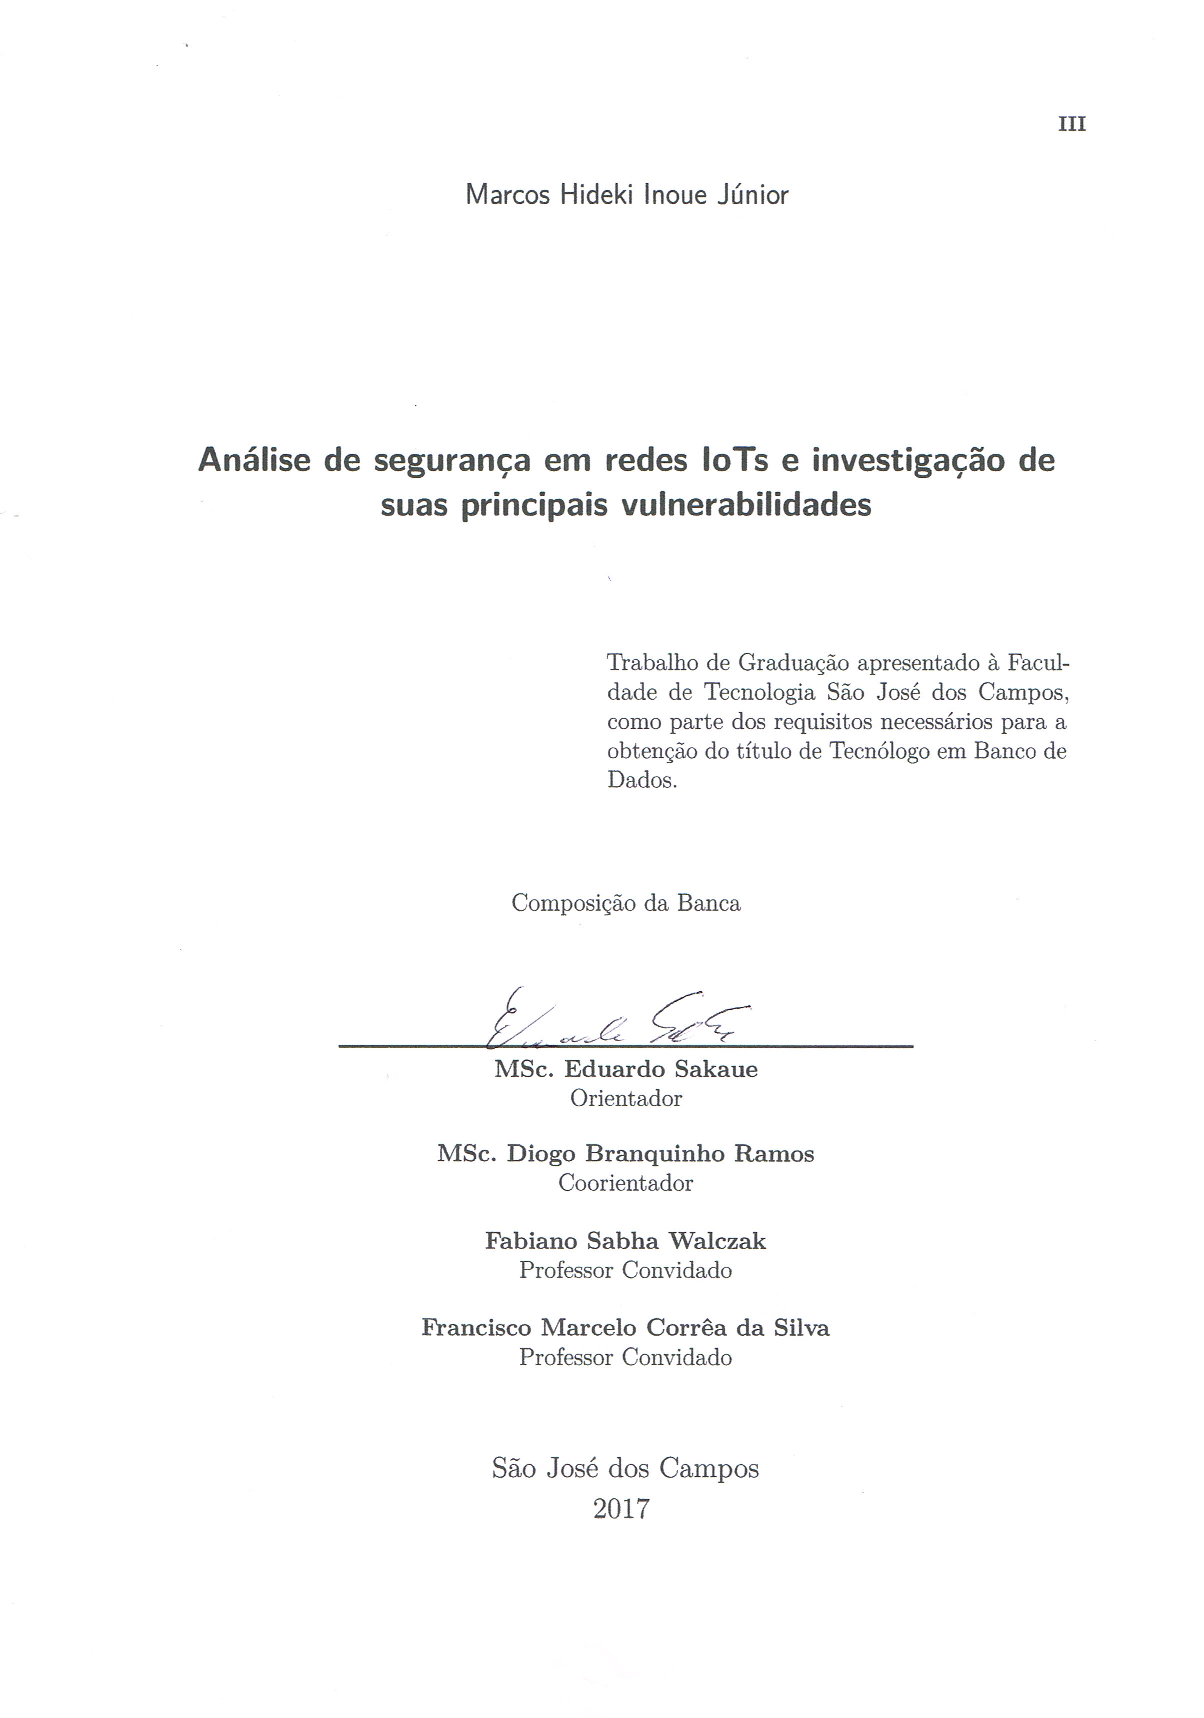
\includepdf[]{folhaAprov.pdf}
% ---

% ---
% Dedicatória
% ---
\include{pre_dedicatoria}
% ---

% ---
% Agradecimentos
% ---
\include{pre_agradecimentos}
% ---

% ---
% Epigrafe
% ---
\begin{epigrafe}
    \vspace*{\fill}
    \begin{flushright}
% Little easter egg. 
%        \textit{''Eu acredito que os HotDogs simbolizam uma filosofia muito profunda, \\
%                na qual todos nós poderíamos ter a oportunidade de observá-la e aprendê-la. \\
%                O pão pode significar tudo que dá a nossa base para a nossa vida. \\
%                E a salsicha pode simbolizar nós mesmos, ou um simples conceito ou coisa que surge de uma epifania.''\\
%                (Rodrigo Takeshi, 26 de Outubro de 2016)}

        \textit{“Epigrafe, citar alguma frase de outra pessoa que tenha rela\~c\~ao com o TG”\\
        (Marcos Hideki)}
    \end{flushright}
\end{epigrafe}
% ---

% ---
% RESUMOS
% ---
% resumo em português
\setlength{\absparsep}{18pt} % ajusta o espaçamento dos parágrafos do resumo
% --- resumo em português ---
\begin{resumo}
    Apresentação concisa dos pontos relevantes do documento deve ser exposta no resumo. No presente caso o resumo será informativo, assim deverá ressaltar o objetivo, a metodologia, os resultados e as conclusões do documento. A ordem desses itens depende do tratamento que cada item recebe no documento original. O resumo deve ser composto por uma seqüência de frases concisas, afirmativas e não em enumeração de tópicos. Deve ser escrita em parágrafo único e espacejamento de 1,5. A primeira frase deve ser significativa, explicando o tema principal do documento. Deve-se usar o verbo na voz ativa e na terceira pessoa do singular. Quanto a sua extensão, o resumo deve possuir de 150 a 500 palavras.   
    \vspace{\onelineskip}
    \noindent
    \textbf{Palavras-chave}: palavras chaves, resumo, português.
\end{resumo}

% resumo em inglês
\begin{resumo}[Abstract]
    \begin{otherlanguage*}{english}
        O abstract é o resumo da obra em língua estrangeira, que basicamente segue o mesmo conceito e as mesmas regras que o texto em português. Recomenda-se que para o texto do abstract o autor traduza a versão do resumo em português e faça, se necessário, os ajustes referentes à conversão dos idiomas. É importante observar que o título e texto NÃO DEVEM estar em itálico.
	    \vspace{\onelineskip}
	    \noindent
	    \\
	    \textbf{Keywords}: Keywords, abstract, english.
    \end{otherlanguage*}
\end{resumo}
% ---

% ---
% inserir lista de ilustrações
% ---
\pdfbookmark[0]{\listfigurename}{lof}
\listoffigures*
\cleardoublepage
% ---

% ---
% inserir lista de tabelas
% ---
\pdfbookmark[0]{\listtablename}{lot}
\listoftables*
\cleardoublepage
% ---

% ---
% inserir lista de abreviaturas e siglas
% ---
\include{pre_lista_siglas}
% ---

% ---
% inserir lista de símbolos
% ---
\include{pre_lista_simbolos}
% ---
% ---
% inserir o sumario
% ---
\pdfbookmark[0]{\contentsname}{toc}
\tableofcontents*
\cleardoublepage
% ---

% ----------------------------------------------------------
% ELEMENTOS TEXTUAIS
% ----------------------------------------------------------

\textual

\setcounter{page}{15}
% ---
% Incluindo Capitulo 1 - Introducao
% ---
% ----------------------------------------------------------
% Introdução (exemplo de capítulo sem numeração, mas presente no Sumário)
% ----------------------------------------------------------
\chapter[Introdução]{Introdução}
%\addcontentsline{toc}{chapter}{Introdução}
% ----------------------------------------------------------
\par O trabalho é motivado pela necessidade / oportunidade de...
\par Apresentar brevemente o problema para explicar a motiva\~c\~ao para o realizar.
\par Recomendável a utilização de figuras e/ou tabelas.

\section{Problema}
\par Apresente claramente o seu problema.

% Section Objetivo Geral!
\section{Objetivo Geral}
\par O objetivo geral deste trabalho é... visando...
\par (...)

% Section Objetivo Especifico!
\section{Objetivo Espec\'ifico}
\par Para a consecução deste objetivo foram estabelecidos os objetivos específicos:
\begin{itemize}
    \item Realizar uma investigação sobre os atuais;
    \item Propor...
    \item (...)
\end{itemize}


% ---

% ---
% Incluindo Capitulo 2 - Fundamentacao Teorica
\chapter{Fundamentação Teórica}
\label{ch:fundamentacao}
\par Neste capítulo ser\~ao fundamentados os conhecimentos b\'asicos para o entendimento do trabalho.

% ---

% ---
% Incluindo Capitulo 3 - Desenvolvimento
	\newpage
\chapter{Desenvolvimento}
\label{ch:desenvolvimento}

\section{Desenvolvimento dessa section}
\par Este capítulo apresenta o processo de desenvolvimento da solução proposta. Seu conteúdo pode variar, dependendo da metodologia adotada.

% ---

% ---
% Incluindo Capitulo 4 - Casos de Testes
\newpage
\chapter{Casos de Testes}
Neste capitulo serão apresentados os testes que foram implementados com a solução e o conteúdo apresentado.

% ---

% ---
% Incluindo Capitulo 5 - Conclusao
    \newpage
\chapter{Conclus\~ao}
Conclusao para o trabalho, mostra como a solu\~c\~ao proposta cumpre com o que foi apresentado anteriormente.
% ---

% ---
% Referências bibliográficas
\bibliography{./ref/referencias}
% ---
\end{document}
